\chapter{Data Analysis and Modelling}

Data is a crucial part of this project, sourced from various publicly available and directly engaged methods to study the evolution of place names accompanying the transformation of Edo into Benin City. Here are the main data sources used:

\begin{enumerate}[label=\arabic*.]
    \item \textbf{Internet Sources:} Old and current maps, and historical documents accessible through publicly available online repositories. These documents include official decrees, land surveys, city plans, and census records, all sourced from public online platforms such as Old Maps of Nigeria and Current Maps of Nigeria.
    \item \textbf{Interviews:} Structured interviews with local historians and community leaders, providing publicly accessible insights and historical context about place names.
    \item \textbf{Surveys:} Surveys distributed to gather contemporary perspectives on historical place names from community members, ensuring direct community engagement.
    \item \textbf{Public APIs:} Integration with publicly available APIs such as OpenStreetMap API to fetch geospatial data and maps.
    \item \textbf{Local Knowledge and Community Engagement:} Direct engagement with local communities to gather oral histories and traditional knowledge about place names through interviews and surveys.
\end{enumerate}

Due to the limited availability of public datasets in Nigeria, I employed alternative strategies, such as sourcing historical documents and conducting text analysis. This approach provided valuable insights despite the data gap.
\section{Analysis of Historical Documents}
Historical documents have been instrumental in unraveling the historical evolution of place names in Edo and Benin City. Analyzing historical documents, maps, and administrative records has highlighted colonial renaming initiatives and their motivations. Indigenous sources, such as oral histories, provided additional perspectives on naming practices. Additionally, the development of a data model and an information system facilitated the management of place name data, including recorded pronunciations.

\subsection{Sources of Data and Processing}
\begin{enumerate}[label=\arabic*.]
    \item \textbf{Historical Documents:}
    \begin{itemize}
        \item \textbf{Sources:} Old maps, colonial records, available administrative archives.
        \item \textbf{Processing:} Processed using data mapping and schema alignment techniques.
    \end{itemize}
    
    \item \textbf{API Data:}
    \begin{itemize}
        \item \textbf{Sources:} Public APIs (e.g., OpenStreetMap) and custom APIs.
        \item \textbf{Processing:} Integrated using API integration techniques, handled rate limiting, and ensured structured data retrieval.
    \end{itemize}
    
    \item \textbf{Manual Data Entry:}
    \begin{itemize}
        \item \textbf{Sources:} Domain experts and collaborators.
        \item \textbf{Processing:} Entered through user-friendly interfaces with validation rules to ensure accuracy and consistency.
    \end{itemize}
    
    \item \textbf{Bulk Data Import:}
    \begin{itemize}
        \item \textbf{Sources:} CSV and Excel files from libraries and local post offices.
        \item \textbf{Processing:} Uploaded in bulk, mapped to the database schema, and converted data types appropriately.
    \end{itemize}
    
    \item \textbf{Preprocessed Data:}
    \begin{itemize}
        \item \textbf{Techniques:} Cleaning (duplicate removal, missing value handling), normalization, error correction, data transformation, integration, validation, enrichment, storage, indexing.
    \end{itemize}
\end{enumerate}

\textbf{The Benin Kingdom Document:}
This document provides an analysis based on the RAFBookletYear-5-1 \href{https://denhamgreenacademy.e-act.org.uk/wp-content/uploads/sites/5/2020/10/RAFBookletYear-5-1Benin-Kingdom-paper-size-297x21-cmUPDATED.210187322-wecompress.com_.pdf}{Benin-Kingdom} and offers significant insights into the historical, cultural, and socio-economic aspects of the Benin Kingdom.

\begin{itemize}
  \item \textbf{Historical Context:} The document outlines the establishment of the Benin Kingdom, highlighting significant events, key rulers, and cultural practices that shaped its history.
  \item \textbf{Cultural Significance:} Key terms such as ``Oba'' (king or chief), ``Ogisos'' (first kings of Benin), ``Voodoo'' (a religion widely followed in Benin), and ``Animism'' (belief in non-human spirits or souls) are explored, shedding light on the religious and social practices prevalent among the Benin people.
  \item \textbf{Chronological Events:} A detailed timeline of events is provided, documenting the chronological development of the Benin Kingdom including the construction of the moat, reigns of notable rulers such as Oba Ewuare the Great, and interactions with European entities like the Portuguese.
  \item \textbf{Geographical Context:} The document discusses various geographical locations such as Edo, Ubinu (Benin in Portuguese), and Igodomigodo, providing insights into the territorial expansion and historical evolution of the kingdom.
  \item \textbf{Trade and Commerce:} Economic aspects are highlighted through references to "Cowrie shells" used as currency and the establishment of trading links with Europeans, illustrating the kingdom's active participation in regional and international trade networks.
  \item \textbf{Social Structure:} Insights into the social structure and political dynamics are provided through mentions of guilds and civil wars, indicating the organizational framework of craftsmen and the internal conflicts within the kingdom.
  \item \textbf{Educational Content:} The document serves as an educational resource, offering foundational knowledge about the history, culture, and geography of the Benin Kingdom, particularly targeted at Year 5 students.
\end{itemize}
\subsubsection{Key Findings}
The tables below summarize key findings based on the text analysis of a historical document. See Table~\ref{tab:vocabulary} for vocabulary terms and their meanings, Table~\ref{tab:timeline} for a timeline of events, and Table~\ref{tab:edo_vocab} for some specific Edo vocabulary.

\begin{table}[htb]
\centering
\caption{Vocabulary of common terms}
\label{tab:vocabulary}
\begin{tabularx}{\linewidth}{|l|X|}
\hline
\textbf{Word} & \textbf{Meaning} \\
\hline
Vocabulary & \\
\hline
Oba & A king, or chief. \\
\hline
Ogisos & The first kings of Benin. Ogisos means “Rulers of the Sky”. \\
\hline
Empire & Lots of countries or states, all ruled by one monarch or single state. \\
\hline
Guild & A group of people who all do the same job, usually a craft. \\
\hline
Animism & A religion widely followed in Benin. \\
\hline
Voodoo & The belief that non-human objects have spirits or souls. They are treated like Gods. \\
\hline
Cowrie shells & A sea shell which Europeans used as a kind of money to trade with African leaders. \\
\hline
Civil war & A war between people who live in the same country. \\
\hline
Moat & A long trench dug around an area to keep invaders out. \\
\hline
\end{tabularx}
\end{table}

\begin{table}[htb]
\centering
\caption{Timeline of Events}
\label{tab:timeline}
\begin{tabularx}{\linewidth}{|l|X|}
\hline
\textbf{Year} & \textbf{Event} \\
\hline
900 CE & Lots of villages join together and make a kingdom known as Igodomigodo, ruled by Ogisos. \\
\hline
900-1460 CE & A huge earthen moat was constructed around the kingdom, stretching 16,000 km long. \\
\hline
1180 CE & The Oba royal family take over from the Osigo, and begin to rule the kingdom. \\
\hline
1440 CE & Benin expands its territory under the rule of Oba Ewuare the Great. \\
\hline
1470 CE & Oba Ewuare renames the kingdom as Edo, with its main city known as Ubinu (Benin in Portuguese). \\
\hline
1485 CE & The Portuguese visit Edo and Ubinu. \\
\hline
1514 CE & Oba Esigie sets up trading links with the Portuguese, and other European visitors. \\
\hline
1700 CE & A series of civil wars within Benin lead to colonization. \\
\hline
\end{tabularx}
\end{table}


\begin{table}[htb]
\centering
\caption{Some Edo-related terms}
\label{tab:edo_vocab}
\begin{tabularx}{\linewidth}{|l|X|}
\hline
\textbf{Term} & \textbf{Definition} \\
\hline
Edo & A member of a people inhabiting the district of Benin in Nigeria. \\
\hline
Igodomigodo & The historical name of the now fallen Benin Empire. \\
\hline
Ogisos & The first kings of Benin. Ogisos means “Rulers of the Sky.” \\
\hline
Oba & A king or chief. \\
\hline
Empire & Lots of countries or states, all ruled by one monarch or single state. \\
\hline
Kingdom & Over a thousand years ago, a group of people known as the Edo lived in West Africa. Around the year 900, the Edo began to cut down trees and make clearings in the rainforests. Lots of villages joined together to make a kingdom known as Igodomigodo, which was ruled by a series of kings, known as the Ogisos or “Rulers of the Sky”. \\
\hline
Voodoo & A religion widely followed in Benin. It combines elements of Roman Catholic ritual with traditional African magical and religious rites. \\
\hline
Animism & The belief that non-human objects have spirits or souls. \\
\hline
\end{tabularx}
\end{table}

\vspace{0.5cm} 
\textbf{Ancient Chronicles:} The investigation of ancient chronicles, such as the "Ife Chronicles" and the "Benin Chronicles," offered foundational accounts of early settlements, legendary narratives, and dynastic histories\cite{otterbein1966}. The ancient chronicles, including the "Ife Chronicles" and the "Benin Chronicles," provide rich accounts of the region's early settlements, legendary narratives, and dynastic histories. According to these chronicles, early settlements were established by legendary figures imbued with divine or semi-divine attributes, signifying their foundational roles in shaping the social and political landscapes of Edo/Benin City. Legendary narratives recount the exploits of these mythical progenitors, depicting their interactions with supernatural beings, the establishment of kinship ties, and the founding of sacred sites. On the other hand, Dynastic histories trace the lineage of ruling families and the succession of kingship within the Edo/Benin polity, highlighting key moments of political consolidation, territorial expansion, and cultural innovation. Through a blend of historical fact and mythic symbolism, these chronicles offer insights into the deep-rooted traditions and cultural heritage underpinning the identity of Edo/Benin City.

\textbf{Colonial Records:} The colonial era ushered in a new era of documentation, with European explorers, missionaries, and administrators recording detailed observations of indigenous societies and governance structures. Archival collections housed in national archives and colonial repositories, including the National Archives of Nigeria and the British Library, yielded valuable correspondence, reports, and surveys shedding light on colonial encounters and administrative reforms in the Edo/Benin region \cite{oliver1985}.

\textbf{Travelogues and Expedition Accounts:} Travelogues and expedition accounts penned by explorers, traders, and ethnographers provided firsthand descriptions of landscapes, settlements, and cultural practices in the Edo/Benin hinterlands. Notable works such as Richard Burton's "A Mission to Gelele, King of Dahomey" and Mary Kingsley's "Travels in West Africa" offered vivid portrayals of local customs, traditions, and historical landmarks\cite{burton2011} and \cite{kingsley1988}.

\textbf{Archaeological Reports:} The rich archaeological heritage of Edo/Benin City yielded a wealth of material culture and stratigraphic data, as documented in archaeological reports and excavation findings. Reports from pioneering archaeologists such as Thurstan Shaw, Graham Connah, and Ekpo Eyo provided crucial insights into ancient Benin's material culture, settlement patterns, and technological advancements\cite{shaw1970,connah1975}.

Archaeological reports from Thurstan Shaw, Graham Connah, and Ekpo Eyo have been instrumental in understanding the transformation of Edo into Benin City. For example, Shaw's 1979 report delved into excavations, revealing evidence of urban planning, architectural structures, and material culture indicative of a burgeoning city. Connah's work from 1975 might have focused on settlement patterns, technological innovations, and social organization within ancient Benin, shedding light on the processes that contributed to its urbanization. Additionally, Eyo's report from 1980 could have provided insights into the stratigraphic data and chronological sequence of cultural developments in the region, offering valuable context for understanding the transition from Edo to Benin City. These archaeological findings collectively contribute to our understanding of the socio-cultural and economic dynamics accompanying the city's transformation over time.

\textbf{Oral Traditions and Indigenous Knowledge:} Recognizing the importance of oral traditions as repositories of collective memory and cultural heritage, I engaged with local communities and indigenous scholars to document oral histories, folk tales, and place-name traditions associated with Edo/Benin City. Transmitted across generations, these narratives offered nuanced perspectives on the socio-cultural dynamics shaping the toponymic landscape. One oral tradition recounted by local communities might involve narratives of migration, conquest, and settlement that contributed to the transformation of Edo into Benin City. For instance, one older man shared stories of legendary figures or ancestral rulers who led their people to establish a new capital, marking the beginning of Benin City's emergence as a prominent political and cultural center. These tales could provide insights into the socio-political processes, power struggles, and symbolic meanings associated with the city's renaming and evolution.

This study focuses on the historical evolution of place names in Edo/Benin City, emphasizing data acquisition and preprocessing to ensure high-quality and reliable data. By analyzing historical documents, we aim to understand the cultural and historical significance of these place names.

\section{Key Findings}
\begin{enumerate}
    \item \textbf{Colonial Influences}: The analysis highlighted significant colonial impacts on place naming practices. Colonial authorities often imposed English or European names on geographical features, urban centers, and administrative districts.
    \item \textbf{Persistence of Indigenous Names}: Despite these changes, indigenous place names persisted in local memory and oral traditions, serving as resilient symbols of cultural heritage and identity.
    \item \textbf{Linguistic Diversity}: The dynamic nature of place naming practices was evident, with linguistic diversity, cultural influences, and historical legacies playing a crucial role in shaping place names.
\end{enumerate}

These findings illustrate the multifaceted nature of place naming practices in Edo and Benin City and contribute to a deeper appreciation of the region's cultural heritage and identity.

\section{Visualization of Place Name Evolution}

Utilizing Geographic Information System (GIS) technology, I embarked on visualizing the evolutionary journey of Edo to Benin City through maps and charts. These visualizations offer a spatial-temporal perspective on the transformation of toponyms over centuries, shedding light on the complex processes and historical events that shaped the city's nomenclature.


\begin{figure}[h!]
    \centering
    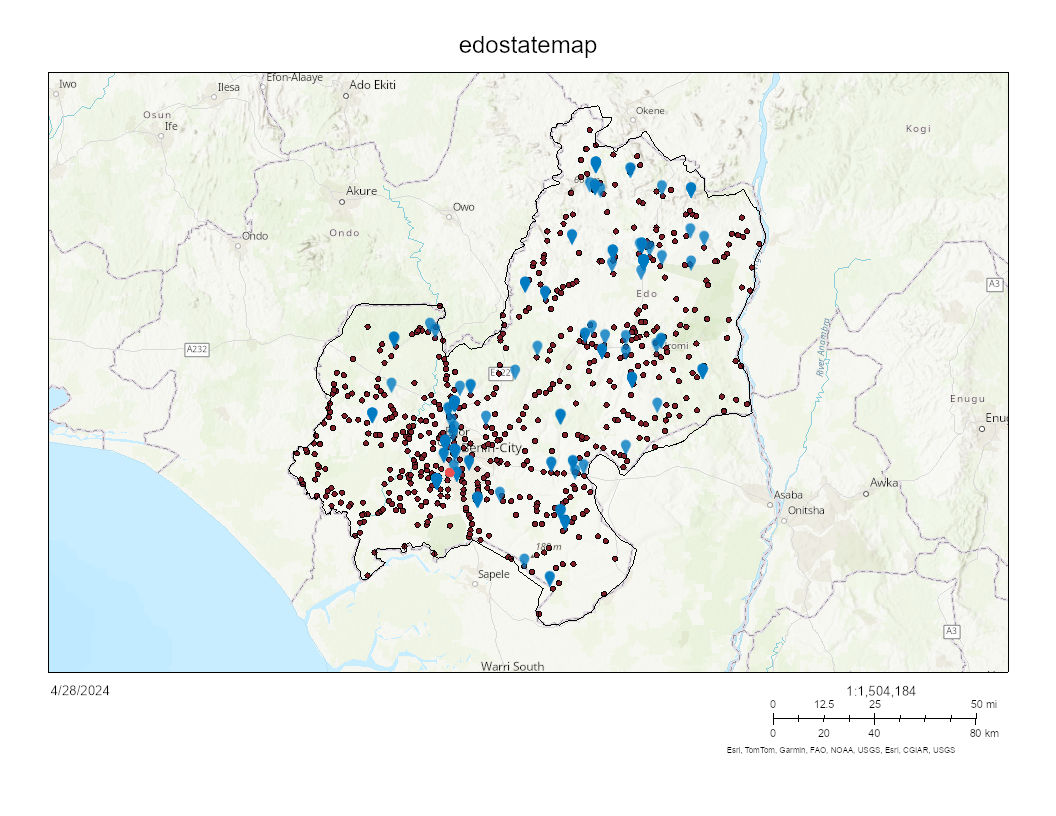
\includegraphics[width=1\linewidth]{edostate_updated.jpg}
    \caption{Map of Edo State}
    \label{fig:edostatemap}
\end{figure}
\vspace{1cm}
\begin{figure}[h!]
    \centering
    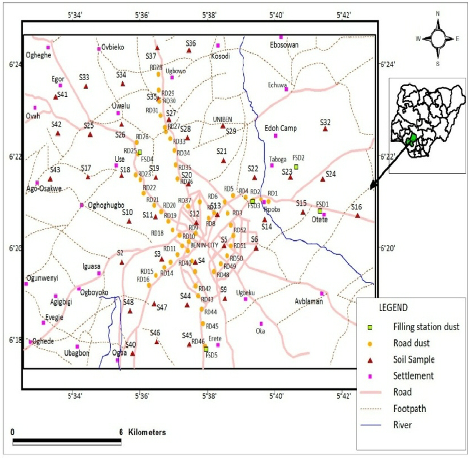
\includegraphics[width=1\linewidth]{edobenin.png}
    \caption{Map of Edo to Benin City}
    \label{fig:edobeninstatemap}
\end{figure}

The figure \ref{fig:edostatemap} and \ref{fig:edobeninstatemap} were generated using data from ArcGIS online using it's available online web application  \href{https://www.arcgis.com/apps/mapviewer/index.html}{here}. All maps are created in compliance with ArcGIS licensing terms.
Detailed processing steps include data extraction, geocoding, and visualization techniques to ensure accuracy and clarity. Geological Map of Edo State: Benin City and Other Locations (Nigerian Geological Survey Agency, 2020). The map depicts the geographical region, including Edo and Benin City, and highlights significant characteristics like rivers, hills, woods, and metropolitan areas. The map distinguishes between indigenous and colonial-era place names by superimposing historical maps on contemporary datasets, using various markers or colors to indicate each.

In addition to the interactive map, I performed several other visualizations with geocoded data to gain further insights into historical place names' spatial distribution and patterns, as shown in the following charts.

\begin{itemize}
    \item The heatmap allows visualization of the density or concentration of historical place names in different areas, which helps identify areas with high concentrations of place names and sparsely populated areas.
\end{itemize}


\begin{figure}[h!]
    \centering
    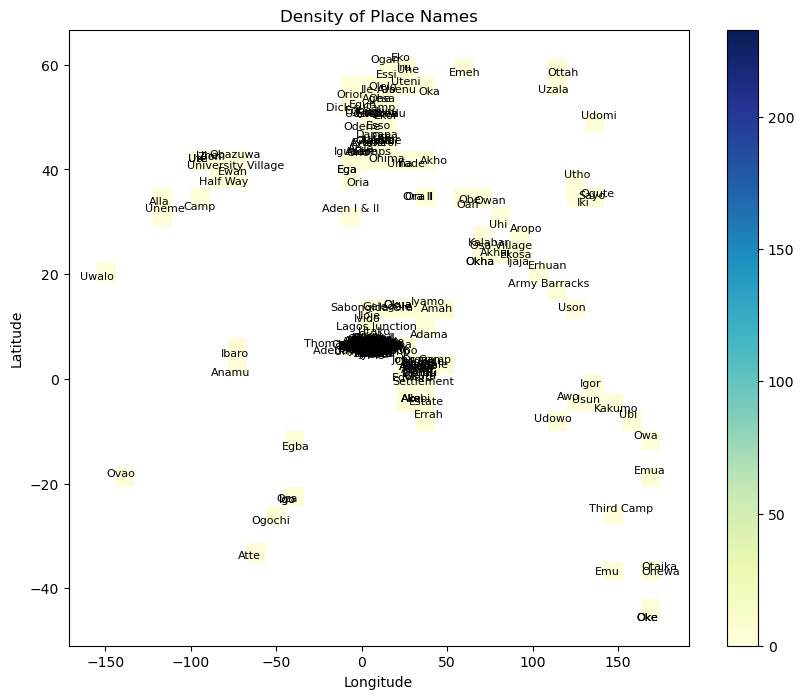
\includegraphics[width=1\linewidth]{heatmap1.png}
    \caption{Heat map presenting density of place names}
    \label{fig:heatmap}
\end{figure}
\newpage
I also plot the histogram of temporal distribution, which provides insight into the frequency of place names across various historical epochs. The dataset is organized into distinct temporal periods, with each bar representing the count of place names associated with a particular timeframe. By analyzing the distribution of bars, one can discern temporal patterns and trends in place-naming practices, identifying periods of heightened activity or significance in naming places. This visualization provides the historical context of place names, shedding light on the evolution and dynamics of naming conventions over time.

\begin{figure}
    \centering
    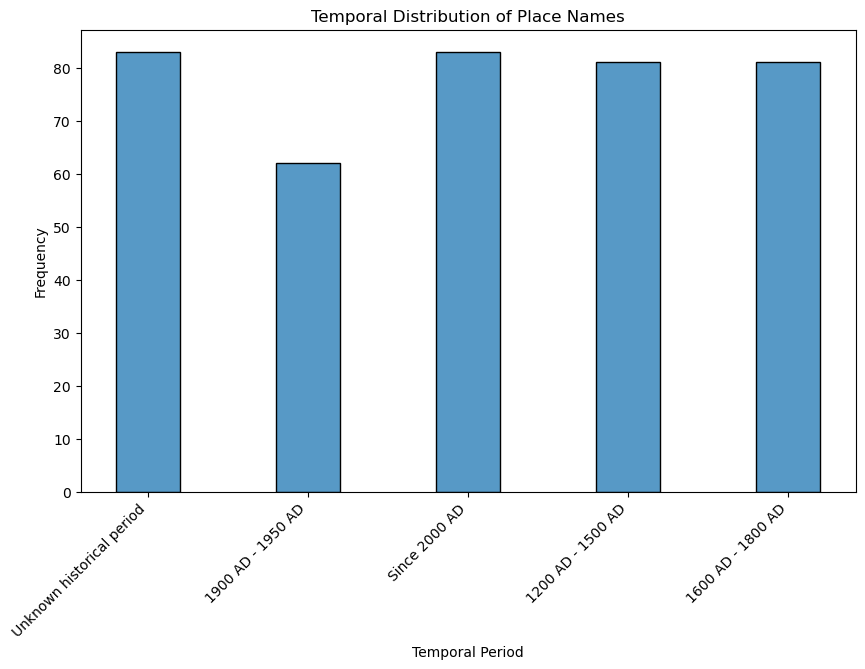
\includegraphics[width=1\linewidth]{output2.png}
    \caption{Temporal Distribution of Place Names}
    \label{fig:histgram}
\end{figure}
\newpage

The histogram shows the top 20 most prevalent village names and their frequency in the dataset. It provides a fast insight into common naming trends by displaying the frequency and distribution of village names in the dataset.

\begin{figure}
    \centering
    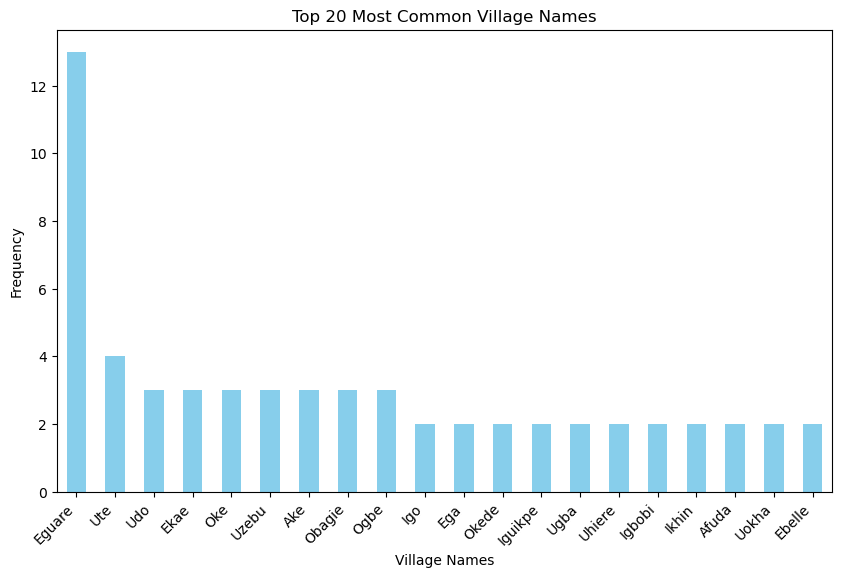
\includegraphics[width=1\linewidth]{histogram2.png}
    \caption{Top 20 Most Common Village Names}
    \label{fig:histogram2}
\end{figure}
\newpage

\begin{figure}
    \centering
    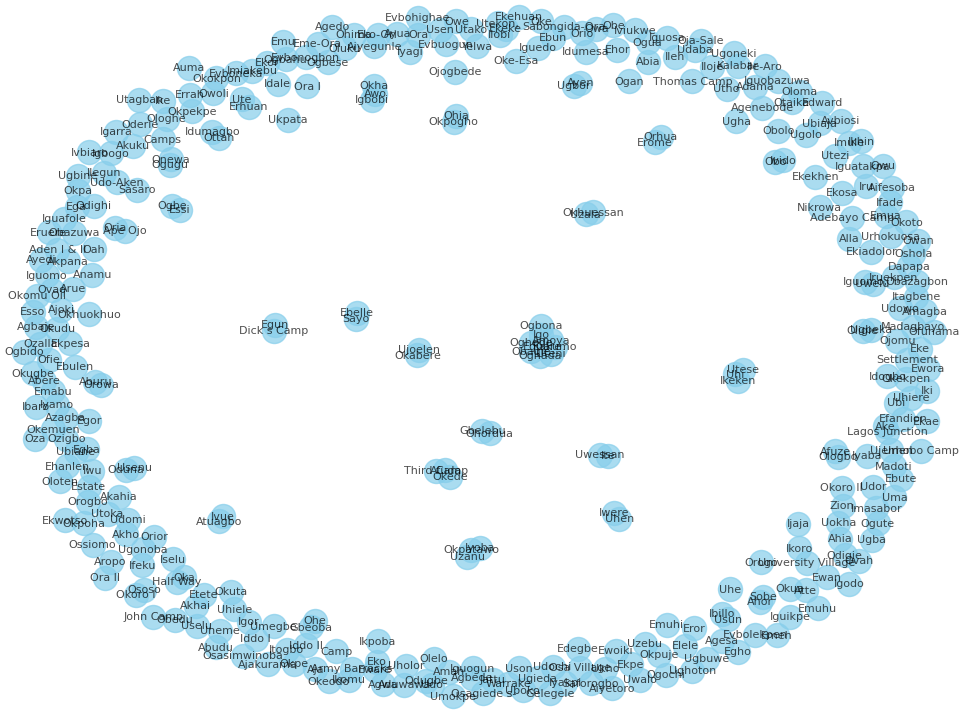
\includegraphics[width=1\linewidth]{networkanalysis.png}
    \caption{Spatial Relationships between Place Names}
    \label{fig:network}
\end{figure}
A network visualization to explore the spatial relationships between place names based on proximity or connectivity has been constructed together with a network graph where nodes represent place names and edges represent spatial connections between them the figure below give insights on the spatial relationships between place names.
\newpage
I create a word cloud visualization to show the frequency or prevalence of terms in place names. This is able to identify recurring themes or patterns in naming conventions.
\begin{figure}
    \centering
    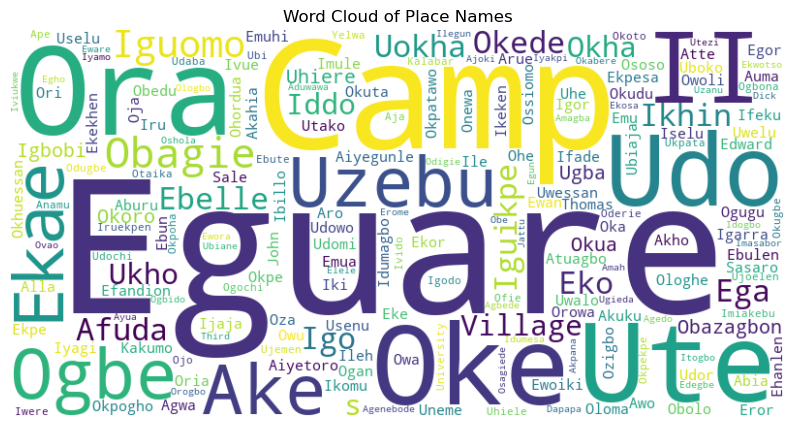
\includegraphics[width=1\linewidth]{wordcloud.png}
    \caption{Word Cloud of Place Names}
    \label{fig:wordcloud}
\end{figure}


\section{Development of Data Models for Place Names Information System}

\subsection{Context and Importance}
The development of data models for the Place Names Information System (PNIS) is pivotal in capturing the historical and geographical evolution of place names in Edo and Benin City. These models facilitate the systematic organization, storage, and retrieval of complex datasets, enabling comprehensive analysis and visualization of toponymic data.

\subsection{Database Schema Design}
The core of the PNIS is a relational database schema encompassing various attributes and relationships of place names and their historical contexts. This schema includes tables for administrative details, geographical features, historical events, and user-generated content. Each table is designed with primary and foreign keys to ensure data integrity and facilitate complex queries. This schema supports the integration of multiple data sources, ensuring that each aspect of place names ranging from administrative details to user-generated content is adequately captured and represented.

\subsubsection{Tables and Attributes}
\begin{itemize}
    \item \textbf{Administrative Details:} This table stores hierarchical administrative information such as local government areas, states, and countries, which are essential for understanding the administrative evolution of place names.
    \item \textbf{Geographical Features:} This table captures data related to the physical characteristics of locations, including type, coordinates, and demographic information. This is crucial for spatial analysis and understanding the geographical context of place names.
    \item \textbf{Historical Data:} This table maintains records of historical events, changes, and narratives associated with each place name, providing a temporal dimension to the data.
    \item \textbf{Alternative Names:} This table includes variations and historical names of places, reflecting linguistic diversity and changes over time.
    \item \textbf{User-Generated Content:} This includes tables for user posts and comments, which allow for community engagement and the incorporation of local knowledge and narratives.
\end{itemize}

\subsubsection{Key Constraints}
\begin{itemize}
    \item \textbf{Primary Keys:} Uniquely identify records in each table ensuring data integrity.
    \item \textbf{Foreign Keys:} Establish relationships between tables, enabling the linkage of related data across different dimensions of the model.
    \item \textbf{Indexes:} Improve query performance, particularly for frequently accessed columns such as location names and geographical coordinates.
\end{itemize}

\section{Procedures Employed}
The development of these data models involved several key methodologies to ensure robustness, scalability, and user accessibility.

\subsection{Normalization}
The database schema was carefully normalized to reduce redundancy and improve data integrity. Normalization ensures that each piece of data is stored only once in the appropriate table and field, facilitating efficient data management and retrieval.

\subsection{Data Mapping and Integration}
\begin{itemize}
    \item \textbf{Schema Mapping:} Aligning data from different sources to the existing database schema was crucial. This involved mapping fields and data types to ensure consistency and accuracy.
    \item \textbf{Data Merging:} Integrating data from multiple sources required resolving conflicts and discrepancies through predefined rules and priority settings.
\end{itemize}

\subsection{Data Preprocessing}
\begin{itemize}
    \item \textbf{Cleaning and Transformation:} Techniques such as duplicate removal, missing value handling, and error correction were employed to ensure high data quality.
    \item \textbf{Feature Engineering:} New features were derived from raw data to enhance the dataset, such as calculating population density from area size and population data.
\end{itemize}

\section{System Capabilities and User Interaction}
The PNIS is designed not only to store and manage data but also to facilitate user interaction and community engagement through a web-based interface.

\subsection{User-Friendly Interface}
The web application, developed using PHP, HTML, CSS, JavaScript, and AJAX, provides an intuitive platform for users to explore and manage place name data. Key features include:

\begin{itemize}
    \item \textbf{Search Functionality:} Allows users to search for locations based on name, postal code, or alternative names, providing quick access to relevant data.
    \item \textbf{Interactive Maps and Visualizations:} GIS integration enables users to visualize place names and their historical evolution on interactive maps.
    \item \textbf{Content Management:} Users can contribute to the dataset by submitting posts and comments about locations. This community-driven approach enriches the dataset with local knowledge and contemporary narratives, ensuring that the database remains dynamic and up-to-date.
\end{itemize}

\subsection{Security and Performance}
\begin{itemize}
    \item \textbf{Role-Based Access Control:} Ensures that only authorized users can perform specific actions, protecting the integrity of the data.
    \item \textbf{Optimized Storage and Indexing:} Enhances the performance of data retrieval and processing, crucial for handling large datasets and ensuring a responsive user experience.
\end{itemize}

\section{Impact of this Model on Managing Toponyms}
The PNIS, through its robust data models and comprehensive system capabilities, significantly aids in managing toponyms by:

\begin{itemize}
    \item \textbf{Preserving Historical Data:} The system captures and preserves the historical trajectories of place names, providing valuable insights into their evolution and the factors influencing these changes.
    \item \textbf{Facilitating Research and Analysis:} Researchers and historians can utilize the system to analyze patterns and trends in place name changes, contributing to a deeper understanding of the socio-political and cultural dynamics at play.
    \item \textbf{Supporting Cultural Heritage:} By documenting and analyzing historical place names, the system contributes to the preservation of cultural heritage and indigenous knowledge, ensuring that these valuable narratives are not lost to time.
    \item \textbf{Enhancing Urban Planning and Policy Making:} The insights gained from the PNIS can inform urban planning and policy-making, promoting sustainable development and cultural preservation within the urban landscape of Benin City.
\end{itemize}

\section{System Life Cycle}
The development of the Place Names Information System (PNIS) follows a structured system life cycle encompassing multiple phases from initial concept to deployment and maintenance. This life cycle ensures that the system is developed efficiently, meets user needs, and maintains high standards of quality and reliability.

\subsection{Requirements Analysis}
\begin{itemize}
    \item \textbf{Objective:} Define the system's functionality, performance, and constraints based on user needs and project goals.
    \item \textbf{Activities:}
        \begin{itemize}
            \item Stakeholder Meetings: Conduct discussions with local historians, researchers, and potential users to gather requirements.
            \item Documentation: Develop detailed requirement specifications covering functional and non-functional aspects.
            \item Feasibility Study: Assess technical and economic feasibility, ensuring the project is viable and aligns with organizational goals.
        \end{itemize}
    \item \textbf{Outcome:} A comprehensive requirements document that outlines the scope, objectives, and functionalities of the PNIS.
\end{itemize}

\subsection{System Design}
\begin{itemize}
    \item \textbf{Objective:} Create a blueprint for the system architecture, detailing how the requirements was implemented.
    \item \textbf{Activities:}
        \begin{itemize}
            \item Conceptual Design: Develop high-level architecture, including data flow diagrams and system architecture diagrams.
            \item Database Design: Design the relational database schema, including tables for administrative details, geographical features, historical data, and user-generated content.
            \item Interface Design: Design user interfaces focusing on usability and accessibility.
            \item Security Design: Plan for data security measures, including user authentication, role-based access control, and data encryption.
        \end{itemize}
    \item \textbf{Outcome:} Detailed design documents, including data models, interface mockups, and security protocols.
\end{itemize}

\subsection{Implementation}
\begin{itemize}
    \item \textbf{Objective:} Translate the design specifications into a working system.
    \item \textbf{Activities:}
        \begin{itemize}
            \item Database Development: Create and populate the relational database using MySQL, ensuring all data models are implemented correctly.
            \item API Integration: Develop and integrate public and custom APIs for data acquisition from sources like OpenStreetMap.
            \item Web Application Development: Develop the web application using PHP, HTML, CSS, JavaScript, and AJAX for dynamic content handling.
            \item Coding Standards: Adhere to coding standards and practices to ensure code quality and maintainability.
        \end{itemize}
    \item \textbf{Outcome:} A functional prototype of the PNIS, including the database, integrated APIs, and a basic web interface.
\end{itemize}

\subsection{Testing}
\begin{itemize}
    \item \textbf{Objective:} Ensure the system functions correctly and meets all specified requirements.
    \item \textbf{Activities:}
        \begin{itemize}
            \item Unit Testing: Test individual components for correct functionality.
            \item Integration Testing: Ensure that different modules and APIs work together seamlessly.
            \item System Testing: Conduct end-to-end testing to verify that the system meets all requirements.
            \item User Acceptance Testing (UAT): Involve stakeholders in testing to validate the system against their expectations and real-world use cases.
            \item Performance Testing: Assess system performance, including load handling and response times.
        \end{itemize}
    \item \textbf{Outcome:} A thoroughly tested system with identified and resolved bugs, ensuring robustness and reliability.
\end{itemize}

\subsection{Deployment}
\begin{itemize}
    \item \textbf{Objective:} Make the system available for use in a production environment.
    \item \textbf{Activities:}
        \begin{itemize}
            \item Server Setup: Configure servers and deploy the database and web application.
            \item Data Migration: Transfer any necessary data from previous systems or manual records.
            \item Deployment Scripts: Create scripts for automated deployment and rollback procedures.
            \item Documentation: Provide user manuals and technical documentation for system administrators and end-users.
        \end{itemize}
    \item \textbf{Outcome:} The PNIS is deployed and accessible to users, ready for operational use.
\end{itemize}

\subsection{Maintenance and Updates}
\begin{itemize}
    \item \textbf{Objective:} Ensure the system remains functional, secure, and up-to-date with evolving user needs and technological advancements.
    \item \textbf{Activities:}
        \begin{itemize}
            \item Monitoring: Implement logging and monitoring to detect and resolve issues proactively.
            \item Bug Fixes: Address any issues reported by users or identified through monitoring.
            \item Updates: Roll out updates and enhancements based on user feedback and changing requirements.
            \item Backup and Recovery: Regularly backup data and have a disaster recovery plan in place.
        \end{itemize}
    \item \textbf{Outcome:} An operational PNIS with ongoing support to ensure long-term usability and reliability.
\end{itemize}

\section{Requirements Specification}
The System Requirements Specification (SRS) is created to provide a comprehensive and detailed description of the Place Names Information System (PNIS). It serves as a blueprint for recording data, describing functionalities, and setting performance and design constraints. This SRS provides a clear understanding of the system's objectives, requirements, and users' expectations, facilitating a systematic approach to development, testing, and deployment. This document will also help maintain consistency and ensure that the application meets user needs and thesis goals.

\subsection{Features}
The model will connect with a database to store and retrieve information about locations, administrative areas, and other related aspects such as historical data, alternative names, geographical attributes, and user-generated information.

\subsubsection{Key Features}
\begin{itemize}
    \item \textbf{Administrative Details Locations:} Provide the foundation for understanding the geographical and administrative context of a location.
    \item \textbf{Alternative Names:} Enhance searchability and discovery by incorporating the various names a location may have.
    \item \textbf{Geographical Features:} Offer a deeper understanding of a location’s physical characteristics.
    \item \textbf{Historical Data:} Enrich locations with stories and events that occurred throughout time.
\end{itemize}

\subsection{Functional Requirements}
\subsubsection{User Management}
\begin{itemize}
    \item Users will be able to register, login, and logout.
    \item The application will authenticate users based on username and password stored securely.
    \item Implement mechanisms to reset forgotten passwords.
    \item An admin user type will exist with elevated privileges.
\end{itemize}

\subsubsection{Location Management}
\begin{itemize}
    \item Users will be able to search for locations based on various criteria (name, postal code, etc.).
    \item The application will display details of a location including its description, founding year (if available), and alternative names.
    \item Allow authorized users to add new locations with descriptions and basic details.
\end{itemize}

\subsubsection{Content Management}
\begin{itemize}
    \item Users will be able to create and submit posts related to locations.
    \item Implement a workflow for approving/rejecting posts by administrators.
    \item Users will be able to view posts associated with specific locations.
    \item Allow users to add comments to existing posts.
\end{itemize}

\subsubsection{Administrative Functions}
\begin{itemize}
    \item Admin users can manage user accounts, update administrative details, and potentially manage other aspects of the data.
\end{itemize}

\subsection{Non-Functional Requirements}
\subsubsection{Performance}
\begin{itemize}
    \item The system shall be capable of handling large volumes of data efficiently.
    \item Data retrieval and query processing shall be optimized for responsiveness.
    \item Algorithms for data acquisition shall be designed for scalability and performance.
\end{itemize}

\subsubsection{Security}
\begin{itemize}
    \item Access to the system shall be role-based with different levels of permissions for users.
    \item Data stored within the system shall be encrypted to ensure confidentiality and integrity.
    \item Measures shall be in place to prevent unauthorized access and data breaches.
\end{itemize}

\subsubsection{Reliability}
\begin{itemize}
    \item The system shall be designed with redundancy and failover mechanisms to ensure high availability.
    \item Data integrity checks shall be performed regularly to detect and prevent corruption.
    \item Backup and recovery procedures shall be implemented to mitigate the risk of data loss.
\end{itemize}

\subsection{Data Model (Database Schematic) Diagram and Description} 
Below is the model schematic diagram that provides overall model functionality features:

\subsubsection{Diagram Descriptions}
\begin{itemize}
    \item \textbf{administrativedetails:} This table likely stores administrative area information such as country, state, and local government.
    \item \textbf{administrative\_ass:} This table might store associations between administrative areas and some identifier (location\_id) during a specific period.
    \item \textbf{admin\_actions:} This table could track actions taken by administrators on the system, including affected users or posts.
    \item \textbf{alternativenames:} This table likely stores alternative names for locations.
    \item \textbf{comments:} This table stores information about comments made on posts, including the content and user who created it.
    \item \textbf{geographicalfeatures:} This table stores geographical features associated with locations, including type, location data, and descriptions.
    \item \textbf{historical\_data:} This table stores historical data/events related to locations, including event descriptions, sources, and dates.
    \item \textbf{locations:} Stores information about specific locations, including name, postal code, founding year, and descriptions.
    \item \textbf{posts:} This table stores posts created by users, including content, approval status, and creation time.
    \item \textbf{users:} This table stores information about users, including username, password, email, profile information, and account status.
\end{itemize}

\newpage

\begin{figure}
    \centering
    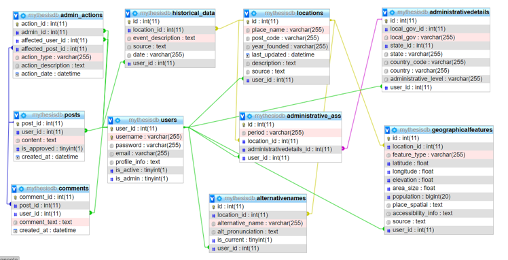
\includegraphics[width=1\linewidth]{model_schema.png}
    \caption{Data Model (Database Schematic) Diagram}
    \label{fig:enter-label}
\end{figure}


\section{Design Specification}
The Place Names Information System (PNIS) is designed to record, manage, and analyze data related to place names and their attributes. The system aims to provide a comprehensive platform for users to explore and learn about various locations in Edo-Benin City. Below is a detailed blueprint of the system architecture, illustrating how the requirements was implemented.

\subsection{System Architecture Overview}
The architecture of PNIS is designed to be modular, scalable, and secure, ensuring that it can efficiently handle large volumes of data and provide a robust user experience. The system is divided into several layers, each responsible for specific functionalities:

\subsubsection{Presentation Layer}
\begin{itemize}
    \item \textbf{Front-End Application:} Developed using HTML, CSS, JavaScript, and AJAX to create a responsive and user-friendly interface. The front-end application will interact with the back-end services through RESTful APIs.
\end{itemize}

\subsubsection{Application Layer}
\begin{itemize}
    \item \textbf{Web Server:} Uses PHP for server-side processing, handling requests from the front end and interacting with the database. The server will manage user sessions, authenticate users, and process CRUD operations.
    \item \textbf{REST API:} Facilitates communication between the front-end application and the database. The API will support operations for user management, location management, and content management.
\end{itemize}

\subsubsection{Data Layer}
\begin{itemize}
    \item \textbf{Database:} A MySQL relational database designed to store and manage all data related to locations, administrative details, user information, and more. The database schema is normalized to reduce redundancy and improve data integrity.
    \item \textbf{Data Acquisition Module:} Handles the integration of data from various sources, including public APIs (e.g., OpenStreetMap), manual data entry, and bulk uploads. This module ensures that data is accurately imported and mapped to the database schema.
\end{itemize}

\subsubsection{Security Layer}
\begin{itemize}
    \item \textbf{Authentication and Authorization:} Implements role-based access control (RBAC) to ensure that only authorized users can access specific features. User passwords are securely stored using hashing algorithms, and JWT is used for stateless authentication.
    \item \textbf{Data Encryption:} Ensures that sensitive data is encrypted both in transit and at rest, maintaining confidentiality and integrity.
\end{itemize}

\subsection{Detailed Implementation of Requirements}

\subsubsection{User Management}
\begin{itemize}
    \item \textbf{Registration and Login:} Users can register with a username, email, and password. The system will validate the input and store the credentials securely. Upon successful registration, users can log in to access their accounts.
    \item \textbf{Password Management:} Provides mechanisms for users to reset forgotten passwords securely through email verification and token-based authentication.
    \item \textbf{Role Management:} Admin users have elevated privileges to manage user accounts, review content, and perform administrative tasks.
\end{itemize}

\subsubsection{Location Management}
\begin{itemize}
    \item \textbf{Search and Discovery:} Users can search for locations using various criteria such as name, postal code, and alternative names. The search functionality will be optimized for quick data retrieval.
    \item \textbf{Location Details:} The application will display detailed information about a location, including its description, founding year, and alternative names. Authorized users can add new locations with relevant details.
\end{itemize}

\subsubsection{Content Management}
\begin{itemize}
    \item \textbf{Post Creation and Submission:} Users can create and submit posts related to specific locations. These posts can include descriptions, historical data, and personal experiences.
    \item \textbf{Approval Workflow:} Administrators will review submitted posts and approve or reject them based on predefined criteria. This ensures that only relevant and accurate content is published.
    \item \textbf{Comments and Interaction:} Users can comment on posts, fostering community interaction and engagement. Comments will be moderated to maintain quality and relevance.
\end{itemize}

\subsubsection{Administrative Functions}
\begin{itemize}
    \item \textbf{User Account Management:} Admin users can manage user accounts, including activating/deactivating accounts and updating user information.
    \item \textbf{Data Management:} Administrators can update administrative details, manage locations, and oversee the overall data integrity.
\end{itemize}

\subsection{Non-Functional Requirements}

\subsubsection{Performance}
The system will be optimized for handling large datasets through indexing, efficient query processing, and caching mechanisms. The data acquisition algorithms are designed to be scalable, ensuring that the system can grow with increasing data volumes.

\subsubsection{Security}
The system employs robust security measures, including role-based access control, data encryption, and regular security audits to prevent unauthorized access and data breaches.

\subsubsection{Reliability}
Redundancy and failover mechanisms are implemented to ensure high availability. Regular data integrity checks and automated backups are performed to prevent data loss and corruption.

\subsection{Data Model (Database Schematic) Diagram}
The database schema is designed to store various attributes of place names and related data:

\begin{itemize}
    \item \textbf{administrativedetails:} Stores administrative information such as country, state, and local government.
    \item \textbf{administrative\_ass:} Associates administrative details with specific locations and periods.
    \item \textbf{admin\_actions:} Tracks actions performed by administrators, including user and post interactions.
    \item \textbf{alternativenames:} Stores alternative names and pronunciations for locations.
    \item \textbf{comments:} Contains user comments on posts.
    \item \textbf{geographicalfeatures:} Records geographical features of locations, including type, coordinates, and descriptions.
    \item \textbf{historical\_data:} Captures historical events and descriptions related to locations.
    \item \textbf{locations:} Central table for storing basic information about locations, including name, postal code, founding year, and descriptions.
    \item \textbf{posts:} Stores posts created by users, including content, approval status, and creation time.
    \item \textbf{users:} Manages user information and authentication details.
\end{itemize}

\section{Implementation of Place Names Information System (PNIS)}
The implementation of the Place Names Information System (PNIS) translates the design specifications into a functional system. This process involves coding, testing, and deploying various components to ensure they work together seamlessly to meet the specified requirements. Here’s a detailed discussion on how the system was implemented.

\subsection{1. Front-End Development}
\begin{itemize}
    \item \textbf{Technologies Used:} HTML, CSS, JavaScript, AJAX
    \item \textbf{User Interface (UI):}
        \begin{itemize}
            \item Developed a responsive and user-friendly interface to allow users to interact with the system. This includes registration, login, location search, and post management functionalities.
            \item Used HTML and CSS for structuring and styling the web pages, ensuring consistency and visual appeal.
            \item Implemented JavaScript and AJAX to handle asynchronous requests, enhancing user experience by dynamically updating content without requiring full page reloads.
        \end{itemize}
    \item \textbf{Search and Navigation:}
        \begin{itemize}
            \item Integrated a search bar that allows users to search for locations using various criteria such as name, postal code, and alternative names. AJAX calls were used to fetch and display results in real-time.
        \end{itemize}
\end{itemize}

\subsection{2. Back-End Development}
\begin{itemize}
    \item \textbf{Technologies Used:} PHP, MySQL, RESTful API
    \item \textbf{Server-Side Logic:}
        \begin{itemize}
            \item Implemented using PHP to handle server-side processing, including user authentication, data processing, and interaction with the database.
            \item Set up RESTful APIs to facilitate communication between the front-end application and the database. These APIs handle CRUD operations for user management, location management, and content management.
        \end{itemize}
    \item \textbf{Database Interaction:}
        \begin{itemize}
            \item Used MySQL as the relational database management system (RDBMS). The database schema was designed to capture relationships between different entities, ensuring data normalization and integrity.
            \item Developed SQL queries and stored procedures to efficiently retrieve and manipulate data based on user inputs and actions.
        \end{itemize}
\end{itemize}

\subsection{3. Data Acquisition and Integration}
\begin{itemize}
    \item \textbf{Technologies Used:} API Integration, Manual Data Entry Interfaces, Bulk Upload Tools
    \item \textbf{API Integration:}
        \begin{itemize}
            \item Integrated with public APIs such as OpenStreetMap to fetch location data. Custom APIs were developed to connect with external data sources, ensuring data is retrieved in a structured and consistent format.
            \item Implemented rate limiting and throttling mechanisms to handle API rate limits and avoid overloading external services.
        \end{itemize}
    \item \textbf{Manual Data Entry:}
        \begin{itemize}
            \item Developed user-friendly interfaces for manual data entry, collaborating with local historians and university researchers to ensure data accuracy and consistency. Validation rules and dropdown selections were implemented to minimize errors.
        \end{itemize}
    \item \textbf{Bulk Data Import:}
        \begin{itemize}
            \item Enabled bulk upload of data files (e.g., CSV, Excel) from trusted sources like libraries and local post offices. Used data mapping techniques to align imported data with the database schema, ensuring proper field matching and type conversion.
        \end{itemize}
\end{itemize}

\subsection{4. Data Preprocessing and Storage}
\begin{itemize}
    \item \textbf{Technologies Used:} Data Cleaning, Transformation, Integration Tools
    \item \textbf{Data Cleaning:}
        \begin{itemize}
            \item Implemented automated scripts and manual review processes to identify and merge duplicate records, handle missing values, and correct errors. Techniques such as imputation and normalization were used to ensure data quality.
        \end{itemize}
    \item \textbf{Data Transformation:}
        \begin{itemize}
            \item Normalized data to fit the relational database schema, ensuring each piece of data is stored in the appropriate table and field. Created new features from raw data to enhance the database, such as calculating population density from area size and population.
        \end{itemize}
    \item \textbf{Data Integration:}
        \begin{itemize}
            \item Merged data from multiple sources, resolving conflicts and discrepancies through predefined rules and priority settings. Schema mapping was used to align data from different sources to the existing database schema.
        \end{itemize}
\end{itemize}

\subsection{5. Security Implementation}
\begin{itemize}
    \item \textbf{Technologies Used:} Encryption, Authentication, Authorization Tools
    \item \textbf{Authentication and Authorization:}
        \begin{itemize}
            \item Implemented role-based access control (RBAC) to ensure only authorized users can perform specific actions. Used bcrypt for password hashing to securely store user passwords.
            \item Employed JSON Web Tokens (JWT) for stateless authentication, ensuring secure user sessions across different parts of the application.
        \end{itemize}
    \item \textbf{Data Encryption:}
        \begin{itemize}
            \item Ensured that sensitive data is encrypted both in transit (using HTTPS) and at rest, maintaining confidentiality and integrity.
        \end{itemize}
\end{itemize}

\subsection{6. Performance and Scalability}
\begin{itemize}
    \item \textbf{Technologies Used:} Caching, Load Balancing, Indexing
    \item \textbf{Performance Optimization:}
        \begin{itemize}
            \item Indexed frequently queried columns to improve data retrieval performance. Implemented caching strategies to store frequently accessed data, reducing database load.
            \item Designed data acquisition algorithms to be scalable, ensuring the system can handle increasing volumes of data without significant performance degradation.
        \end{itemize}
    \item \textbf{Scalability:}
        \begin{itemize}
            \item Implemented load balancing to distribute incoming traffic across multiple servers, ensuring high availability and performance. The system was designed with redundancy and failover mechanisms to maintain reliability.
        \end{itemize}
\end{itemize}

\subsection{7. Testing and Deployment}
\begin{itemize}
    \item \textbf{Technologies Used:} Automated Testing Tools, Continuous Integration/Continuous Deployment (CI/CD)
    \item \textbf{Testing:}
        \begin{itemize}
            \item Conducted unit testing, integration testing, and system testing to ensure all components function correctly. Automated testing tools were used to streamline the testing process and identify issues early.
            \item Performed user acceptance testing (UAT) to gather feedback from end-users and make necessary adjustments.
        \end{itemize}
    \item \textbf{Deployment:}
        \begin{itemize}
            \item Used CI/CD pipelines to automate the deployment process, ensuring that new features and updates are quickly and reliably released. Deployed the system on a cloud platform to ensure scalability and availability.
        \end{itemize}
\end{itemize}




\section{conclusion}
The developed Place Names Information System successfully manages and explores the historical evolution of place names in Edo/Benin City. By integrating historical research with IT tools, the study provides a valuable resource for understanding the cultural and historical significance of place names. The system's capabilities in data acquisition, preprocessing, and user interaction ensure it is a robust tool for managing toponyms, aligning with the declared goals of the thesis.